\section{Motivation}

\subsection{Archipelago}
\begin{frame}{VM Volume storage}
\begin{center}
    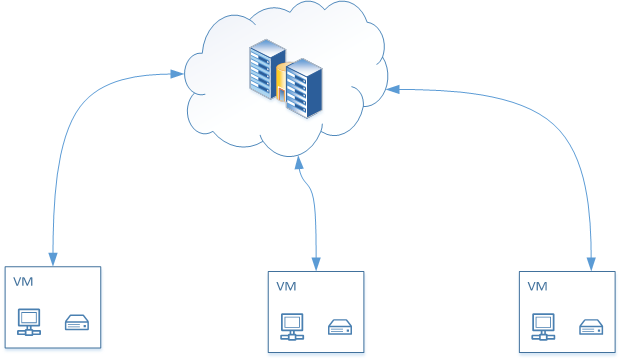
\includegraphics[scale=0.5]{images/cloud-storage.png} \\
\end{center}
\end{frame}

\begin{frame}{Archipelago I}
A thin distributed storage layer aiming to:
\hfill \\
\hfill \\
\hfill \\
\begin{itemize}
\item Decouple storage logic from the actual data store
\item Provide logic for thin cloning and snapshotting
\item Provide logic for deduplication
\item Provide different endpoint drivers to access Volumes and Files
\item Provide backend drivers for different storage technologies
\end{itemize}
\end{frame}

\begin{frame}{Archipelago II}
\begin{center}
    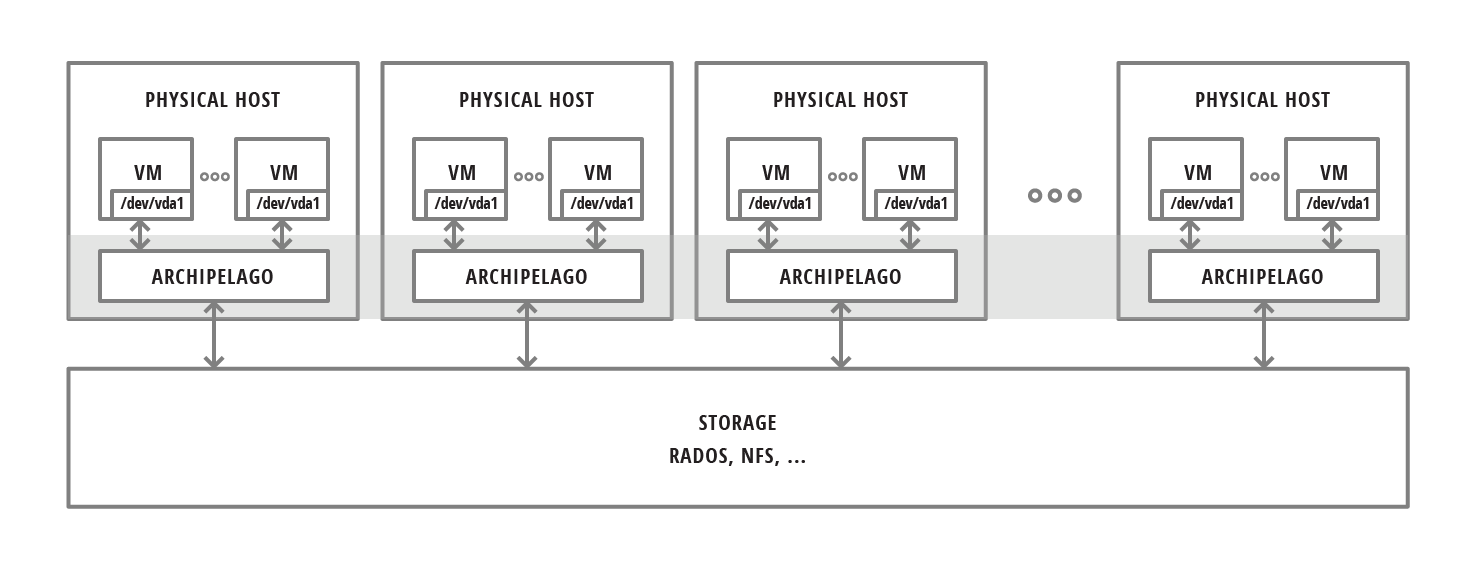
\includegraphics[scale=0.4]{images/archipelago-overview.png} \\
\end{center}
\end{frame}


\begin{frame}{Archipelago III}
\begin{center}
    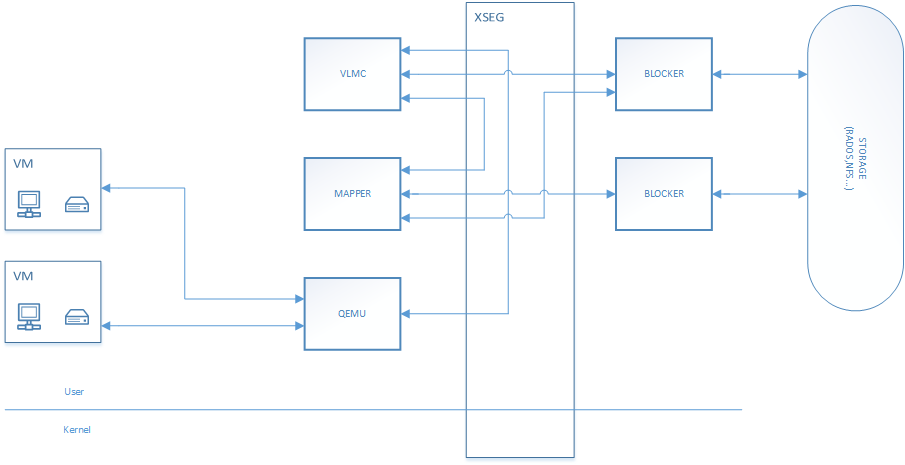
\includegraphics[scale=0.4]{images/archip-comm.png} \\
\end{center}
\end{frame}

\subsection{Distributed storage}

\begin{frame}{RADOS}
is the storage component of Ceph 
\hfill \\
\hfill \\
\hfill \\
\hfill \\

RADOS basic characteristics are:
\begin{itemize}
\item \textit{Replication}
\item \textit{Fault tolerance}
\item \textit{Self-management}
\item \textit{Scalability}\end{itemize}
\end{frame}


\begin{frame}{Storage Abstraction}
\begin{center}
    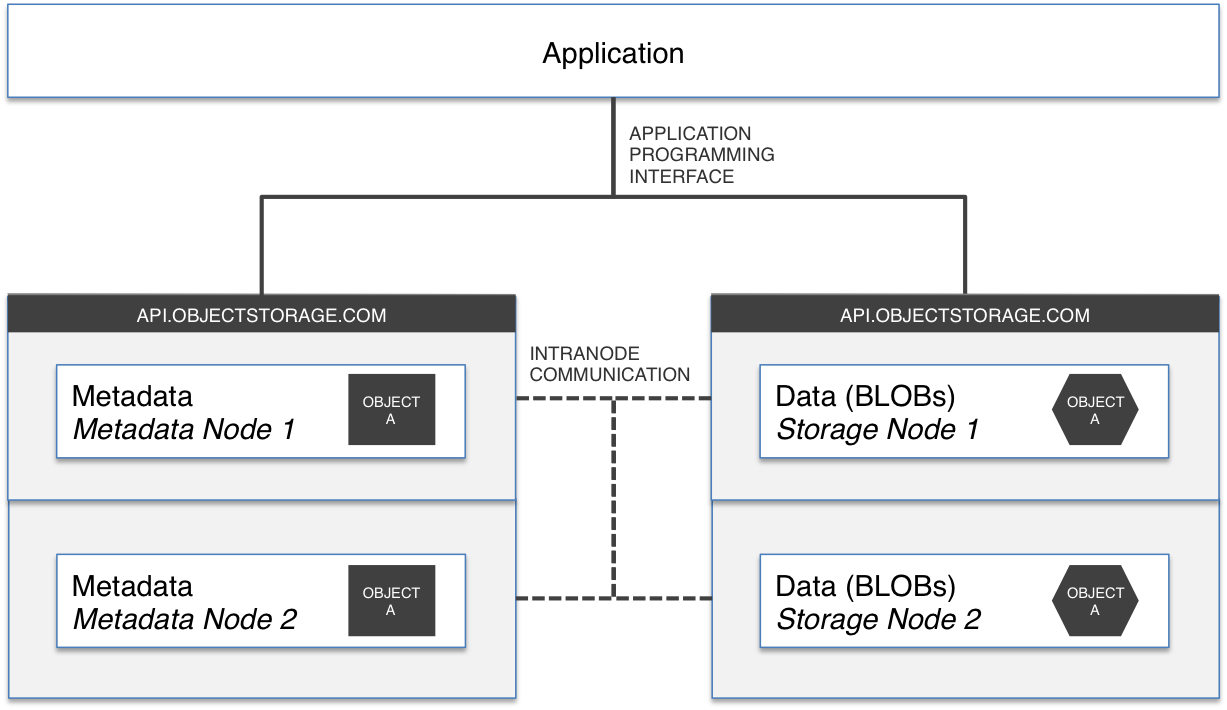
\includegraphics[scale=0.4]{images/object_storage_arch.png} \\
\end{center}
\end{frame}

\subsection{BlkKin}
\begin{frame}{The Problem}
\begin{itemize}
\item Complex service oriented architectures
\item Difficult debugging
\item Difficult monitoring
\item Non-deterministic execution
\item Context-bound faults
\end{itemize}
\end{frame}

\begin{frame}{Solution}
\begin{center}
Distributed end-to-end tracing 
\hfill \\
\hfill \\
 \& 
\hfill \\
\hfill \\
Central data collection
\end{center}
\end{frame}

\begin{frame}{BlkKin}

A distributed tracing infrastructure to track the IO request from Qemu until
RADOS
\hfill \\
\hfill \\
\hfill \\

BlkKin main characteristics:
\begin{itemize}
\item low-overhead tracing 
\item live-tracing
\item End-to-end tracing of causal relationships
\item User interface
\end{itemize}
\end{frame}
